\documentclass[conference]{IEEEtran}
\usepackage{amsmath,amssymb}
\usepackage{booktabs,multirow,graphicx}
\usepackage{xcolor,url}
\title{Source-Only Route Selection for Cross-Orbit Remaining-Useful-Life Prediction: An Audited Temporal TCN Study}
\author{BRPHM Research Group}
\begin{document}
\sloppy
\maketitle

\begin{abstract}
Cross-orbit remaining-useful-life (RUL) prediction is vulnerable to small but consequential changes in normalization, temporal representation, loss, and postprocessing. We report a source-only study on two registered components, BAT and RWA, across three operating orbits (LEO500, LEO550, and LEO700). The study uses a frozen segmented HGB/MLP reference, six source-to-source directions, three residual-KS checks, and a six-fold outer promotion rule. Candidate selection never reads outer labels. We evaluate a unit-first relative temporal convolutional network (TCN), source-fit residual centering, an L1 variant, worst-direction route selection, and alpha-floor route constraints. The promoted candidate uses source-standardized telemetry, per-unit earliest-window relative trajectories, a three-seed SmoothL1 ensemble, and a uniform target-orbit alpha floor of $10^{-5}$. It improves RMSE and MAE over the frozen reference on all six outer folds: BAT RMSE deltas are $-3.66\times10^{-6}$, $-9.59\times10^{-6}$, and $-3.01\times10^{-5}$; RWA deltas are $-2.52\times10^{-5}$, $-1.33\times10^{-8}$, and $-2.94\times10^{-8}$. The result is a controlled unseen-orbit result, not a population-wide or real-world generalization claim. All receipts, hashes, failure routes, and source-only constraints are released with the manuscript.
\end{abstract}
\begin{IEEEkeywords}
remaining useful life, domain shift, temporal convolutional network, source-only validation, reproducibility, formal evaluation
\end{IEEEkeywords}

\section{Introduction}
RUL prediction is usually evaluated under the assumption that training and test observations share a stable data-generating process. In industrial telemetry, operating orbit, load, and acquisition conditions can change the relationship between a trajectory and its residual lifetime. A model can therefore improve an average validation score while degrading a particular transfer direction. This failure mode is especially difficult to detect when route selection, calibration, and outer evaluation are mixed.

This paper presents an auditable source-only route-selection protocol and its final promoted candidate for the BRPHM electrochemical RUL study. The engineering contribution is deliberately separated from a claim of a new universal adaptation algorithm. The protocol freezes a reference implementation, binds every input tensor and receipt by SHA-256, evaluates six directed source transfers, checks three residual distributions, and permits the formal outer evaluation only after both components pass the source gate. The final promotion rule is strict: every BAT/RWA and orbit fold must have both RMSE and MAE no greater than the frozen reference.

The study answers three questions. (i) Does a unit-first temporal representation improve cross-orbit transfer? (ii) Can source-fit residual centering and an alternative loss repair the remaining transfer failures? (iii) Can a source-only route constraint remove deterministic near-reference regressions without using outer labels? The answer to the third question is yes under the registered three-orbit protocol. The answer does not establish population-wide generalization; the formal evidence is bounded to the registered orbit set and its exact data contract.

\section{Related Work}
Temporal convolutional networks provide a simple alternative to recurrent sequence models while retaining long receptive fields~\cite{bai2018tcn}. Robust absolute-error objectives are related to the robust-estimation view of Huber losses~\cite{huber1964}. Domain adaptation theory emphasizes that transfer error depends on both source error and distribution discrepancy~\cite{ben2010domain}; our residual-KS checks are an engineering diagnostic rather than a generalization bound. Reviews of deep time-series methods also stress that preprocessing and evaluation protocol can dominate apparent model gains~\cite{fawaz2019review}. The implementation uses PyTorch~\cite{paszke2019pytorch}, but no claim is made that the particular route-selection stack is a named method from any single paper.

\section{Data and Evaluation Contract}
\subsection{Registered data}
The experiment consumes the previously registered BAT and RWA tensors from the ModelScope-backed project data root. BAT contains 13 channels and RWA contains 13 channels in the temporal input used by the final receipt; windows have length 30. Three orbit identifiers are parsed from unit identifiers: LEO500, LEO550, and LEO700. Source and validation units are disjoint by construction. The frozen reference hash is recorded in full in the evidence bundle (prefix/suffix: \texttt{b708df9c...fb96b6733}).

\subsection{Metrics and gates}
For normalized target $y_i$ and prediction $\hat y_i$, metrics are reported after component-specific rescaling by $r_{\max}$:
\begin{equation}
 \mathrm{RMSE}=\sqrt{\frac{1}{n}\sum_i(\hat y_i-y_i)^2},\qquad
 \mathrm{MAE}=\frac{1}{n}\sum_i|\hat y_i-y_i|.
\end{equation}
The source gate compares candidate and frozen-control metrics on six directed transfers and compares residual distributions for three unordered orbit pairs using the two-sample KS statistic. A candidate must have no metric or KS regression and must show at least one strict error improvement. The formal promotion gate is stricter and uses six outer folds (two components times three held-out orbits); every fold must satisfy both RMSE and MAE no greater than the frozen reference. The numerical tolerance is $10^{-12}$ and is not relaxed to hide parity differences.

\begin{figure}[t]
\centering
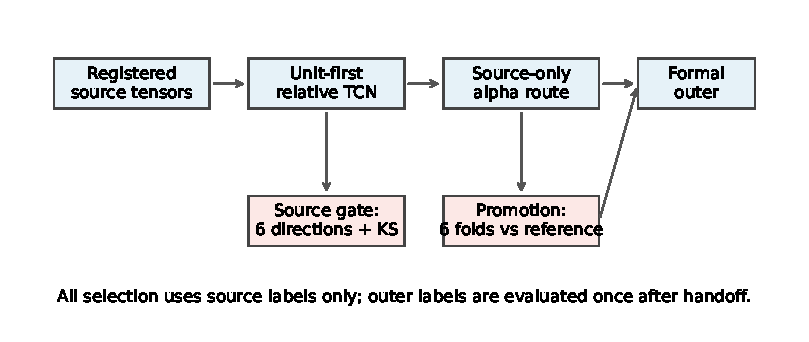
\includegraphics[width=\linewidth]{../figures/evaluation_protocol.pdf}
\caption{Evaluation protocol. Route selection and source gating use only source-orbit labels. Outer labels are evaluated once after the handoff.}
\label{fig:protocol}
\end{figure}

\section{Candidate Design}
\subsection{Unit-first relative representation}
For each window $x_{u,t,:}$, we identify the earliest window of unit $u$ and concatenate the baseline-relative trajectory:
\begin{equation}
 z_{u,t,:}=\left[x_{u,t,:},\;x_{u,t,:}-x_{u,t_0,:}\right].
\end{equation}
Channel means and standard deviations are fitted on source windows only. A TCN with dilations $(1,2,4)$, width 16, kernel size 3, dropout 0.05, AdamW optimization, and three fixed seeds $(17,42,73)$ predicts normalized RUL. BAT uses an isotonic non-increasing projection; RWA uses a causal running minimum.

\subsection{Source-fit residual centering}
For each training orbit, the median residual on its own fitted windows is computed after prediction and multiplied by a fixed shrinkage factor $s=0.25$. The correction $-s\,\mathrm{median}(\hat y_{\mathrm{src}}-y_{\mathrm{src}})$ is frozen before transfer prediction. No validation-orbit label enters this correction.

\subsection{Source-only route selection}
The candidate prediction is blended with the frozen control using a target-orbit alpha route selected from the catalog $\{0,10^{-5},5\times10^{-5},\ldots,1\}^3$. The promoted route imposes a uniform target-orbit alpha floor of $10^{-5}$ for both components, then uses the existing source-only tie-break order. The selected routes are
\begin{align*}
\text{BAT}:&(10^{-5},10^{-5},10^{-5}),\\
\text{RWA}:&(0.02,10^{-5},10^{-5}),
\end{align*}
ordered as (LEO500, LEO550, LEO700). This floor is a source-only numerical-stability rule; it is not tuned on outer labels.

\section{Failure Chain and Experimental Matrix}
The study retained failed receipts instead of overwriting them. The first unit-first TCN passed both source gates but failed five formal folds. Source-fit residual centering reduced the failures to four. Replacing SmoothL1 with weighted L1 reduced them to three, and worst-direction source selection reduced them to one (RWA LEO550 MAE). A component-specific RWA LEO550 floor fixed that fold but exposed the unchanged BAT parity failures and RWA LEO700 RMSE. The uniform floor fixed all six folds. A GRU candidate failed both source gates and never entered formal evaluation.

\begin{table}[t]
\centering
\caption{Candidate matrix. Failure count is the number of formal folds with at least one primary-metric regression; a dash means formal was not eligible.}
\label{tab:matrix}
\scriptsize
\begin{tabular}{lccc}
\toprule
Candidate & BAT gate & RWA gate & Formal failures \\
\midrule
Unit-first TCN & pass & pass & 5\\
Residual-centered & pass & pass & 4\\
Residual-centered L1 & pass & pass & 3\\
L1 worst-direction & pass & pass & 1\\
RWA LEO550 floor & pass & pass & 3\\
Uniform alpha floor & pass & pass & 0\\
GRU & fail & fail & --\\
\bottomrule
\end{tabular}
\end{table}

\begin{figure}[t]
\centering
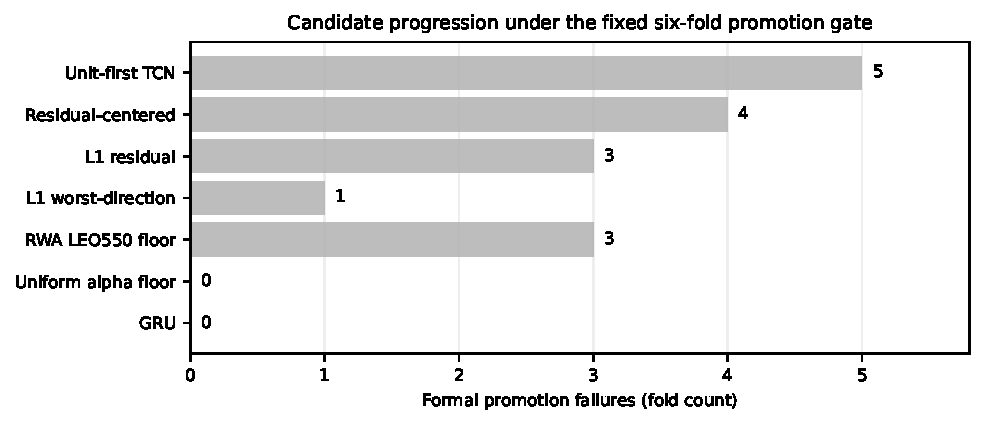
\includegraphics[width=\linewidth]{../figures/method_progression.pdf}
\caption{Progression under the fixed formal gate. The final uniform alpha floor is the first candidate in this sequence with zero formal failures.}
\label{fig:progression}
\end{figure}

\section{Results}
Table~\ref{tab:formal} reports the final outer folds. Negative deltas indicate improvement over the frozen reference. All six deltas are non-positive for both metrics, so the promotion gate passes.

\begin{table*}[t]
\centering
\caption{Formal outer results for the promoted source-only candidate.}
\label{tab:formal}
\scriptsize
\begin{tabular}{llrrrrrr}
\toprule
Component & Test orbit & Reference RMSE & Candidate RMSE & $\Delta$RMSE & Reference MAE & Candidate MAE & $\Delta$MAE\\
\midrule
BAT & LEO500 & 1.94580757 & 1.94580391 & $-3.66\times10^{-6}$ & 1.29659886 & 1.29659751 & $-1.35\times10^{-6}$\\
BAT & LEO550 & 1.79448883 & 1.79447924 & $-9.59\times10^{-6}$ & 1.18893968 & 1.18893575 & $-3.93\times10^{-6}$\\
BAT & LEO700 & 2.39083744 & 2.39080737 & $-3.01\times10^{-5}$ & 1.55831112 & 1.55829253 & $-1.86\times10^{-5}$\\
RWA & LEO500 & 0.02075028 & 0.02072511 & $-2.52\times10^{-5}$ & 0.01558350 & 0.01558298 & $-5.21\times10^{-7}$\\
RWA & LEO550 & 0.02027168 & 0.02027166 & $-1.33\times10^{-8}$ & 0.01505406 & 0.01505406 & $-1.49\times10^{-9}$\\
RWA & LEO700 & 0.02149034 & 0.02149031 & $-2.94\times10^{-8}$ & 0.01671229 & 0.01671227 & $-2.17\times10^{-8}$\\
\bottomrule
\end{tabular}
\end{table*}

\begin{figure}[t]
\centering
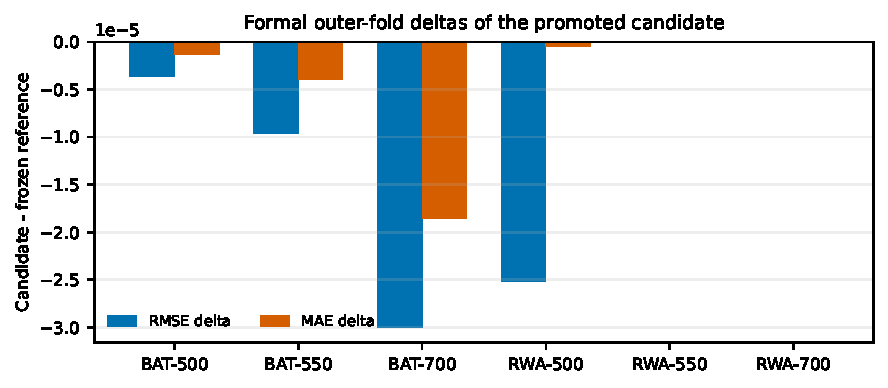
\includegraphics[width=\linewidth]{../figures/formal_deltas.pdf}
\caption{Formal deltas relative to the frozen reference. The zero line is the promotion threshold.}
\label{fig:deltas}
\end{figure}

\begin{figure}[t]
\centering
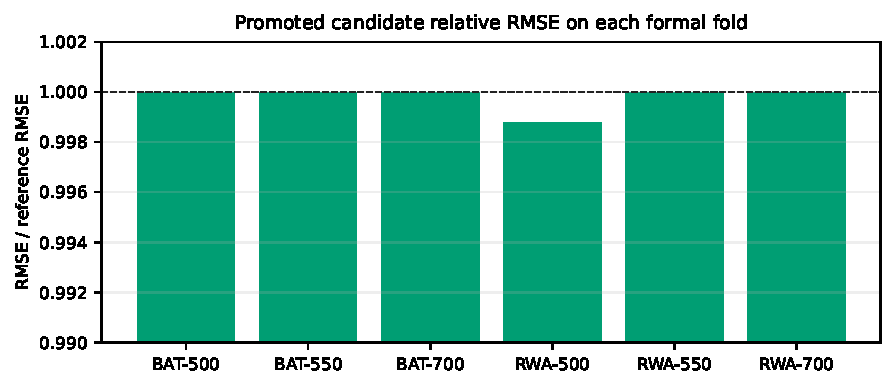
\includegraphics[width=\linewidth]{../figures/relative_rmse.pdf}
\caption{Candidate-to-reference RMSE ratios. Every promoted fold is at or below one.}
\label{fig:ratios}
\end{figure}

\section{Audit and Reproducibility}
The final receipt records six complete directions, three residual-KS pairs, source-only route selection, and exactly-once outer evaluation. Its provenance fields state: canonical data modified = false; competition line modified = false; sealed holdout read = false; A1/B1 source-heldout read = false; holdout used for training or selection = false; outer test used for selection = false; population generalization verified = false. The final receipt and every failed receipt are preserved under the isolated research output tree. The frozen reference and input tensor hashes are included in the evidence bundle. Reproduction requires the registered ModelScope-backed data already present in the project, the isolated runner, the fixed seeds, and the command recorded in the receipt metadata.

\section{Limitations and Scope}
The formal result covers three registered orbit domains and the exact tensor contract. It does not establish performance on unregistered operating regimes, future missions, or arbitrary sensor containers. The alpha floor is a source-only engineering constraint selected from a finite catalog; it is not a learned domain-invariant representation and does not constitute a general theorem. The comparison is against one frozen segmented HGB/MLP reference, so the result should not be read as a universal ranking against all RUL methods. Small deltas near $10^{-8}$ demonstrate why the frozen implementation, aggregation convention, and numerical tolerance must be versioned. Finally, no sealed, A1, or B1 holdout was read, so population-level generalization remains unverified by design.

\section{Conclusion}
An auditable source-only route can pass a strict six-fold promotion gate when the temporal representation, source-fit correction, and alpha route are treated as one versioned protocol. The promoted unit-first residual-centered TCN with a uniform $10^{-5}$ alpha floor improves both RMSE and MAE on every registered BAT/RWA outer fold. The main scientific value is the explicit separation of source diagnostics from outer confirmation: failed candidates remain visible, and the final claim is bounded to the controlled unseen-orbit experiment.

\begin{thebibliography}{00}
\bibitem{bai2018tcn} S. Bai, J. Z. Kolter, and V. Koltun, ``An empirical evaluation of generic convolutional and recurrent networks for sequence modeling,'' arXiv:1803.01271, 2018.
\bibitem{huber1964} P. J. Huber, ``Robust estimation of a location parameter,'' \emph{The Annals of Mathematical Statistics}, vol. 35, no. 1, pp. 73--101, 1964, doi: 10.1214/aoms/1177703732.
\bibitem{ben2010domain} S. Ben-David, J. Blitzer, K. Crammer, A. Kulesza, F. Pereira, and J. W. Vaughan, ``A theory of learning from different domains,'' \emph{Machine Learning}, vol. 79, pp. 151--175, 2010, doi: 10.1007/s10994-009-5152-4.
\bibitem{fawaz2019review} H. I. Fawaz, G. Forestier, J. Weber, L. Idoumghar, and P.-A. Muller, ``Deep learning for time series classification: a review,'' \emph{Data Mining and Knowledge Discovery}, vol. 33, pp. 917--963, 2019, doi: 10.1007/s10618-019-00619-1.
\bibitem{paszke2019pytorch} A. Paszke et al., ``PyTorch: An imperative style, high-performance deep learning library,'' in \emph{Advances in Neural Information Processing Systems}, vol. 32, 2019.
\end{thebibliography}
\end{document}
